\documentclass[10pt,a4paper]{article}
\usepackage[margin=2cm,top=1.8cm,bottom=1.8cm]{geometry}
\usepackage[T1]{fontenc}\usepackage{lmodern}\usepackage{microtype}
\usepackage{graphicx,booktabs,caption,tikz,float,array,tabularx}
\usetikzlibrary{arrows.meta,positioning,shapes.misc,calc}
\captionsetup{font=small,labelfont=bf,skip=4pt}
\usepackage[hidelinks]{hyperref}
\setlength{\parskip}{2pt}\setlength{\parindent}{1em}
\usepackage{titlesec}\titlespacing*{\section}{0pt}{8pt}{3pt}\titlespacing*{\subsection}{0pt}{5pt}{2pt}
\titleformat{\section}{\normalfont\large\bfseries}{\thesection}{0.6em}{}
\titleformat{\subsection}{\normalfont\normalsize\bfseries}{\thesubsection}{0.6em}{}
\graphicspath{{figures/}}
\newcommand{\ok}{\textbf{done}}\newcommand{\no}{\textbf{not done}}
\title{\vspace{-1.2cm}\Large Report 2026-09-24. Campaign run 2:\\a language model as one MATSim replanning strategy\\\large What was achieved, what was not, and what the model actually decides}
\author{\normalsize Giulio Iannelli, MATSim AI Lab.\\\normalsize Repository \texttt{matsim-ai-lab}, branch \texttt{migrate/contrib-llm}, code at commit \texttt{a916897}}
\date{\normalsize Run of 23 September 2026, 16:30--19:36. Report written 24 September 2026. Series: persona-emergence reports, no.~1.}
\begin{document}\maketitle\vspace{-0.9cm}

\section*{Summary}
\noindent MATSim simulates a city day after day. Each synthetic traveller keeps a few daily plans, executes one, gets a score for it and occasionally changes it with a rule-based strategy until the population settles. In this run, for 200 of 8,460 travellers, that strategy was a local 27-billion-parameter language model (LLM) that reads the day in the first person and decides per trip which mode to use. MATSim then scores the result like any other plan. The run: 25 iterations, 10 LLM queries per iteration, 3\,h\,06\,min.

\begin{tabularx}{\textwidth}{@{}>{\bfseries}p{2.3cm}X@{}}
Achieved & The protocol is reliable and fast enough: 250 of 250 queries gave a valid, physically checked decision in one model round, 39\,s median. The panel and trigger logic behaved as designed. The population stayed at rest, so the LLM's effect is readable per agent. The reasoning is in the first person and grounded in the stated traits in 78\,\% of conversations. \\[2pt]
Not achieved & No behavioural result. The model's decision is a near-deterministic rule (a car owner drives, everyone else keeps the bus), so age, job and travel times modulate the narrative, not the choice. No learning: 20,799 experience facts were written to the vector store and none reached a prompt. MATSim's scoring neither confirmed nor rejected the switches (car and bus score alike). No effect on the population, by design. \\[2pt]
Issues & A context bug in the first attempt silently forbade every car switch (fixed, run repeated). A colleague's job on the shared GPU forced a model reload in 117 of 250 queries (25\,\% of LLM time). The analysis suite does not understand the new decision format. Departure-time changes were never used. \\
\end{tabularx}

\section{Setting and question}
Every MATSim agent owns up to six plans (a chain of activities with trips between them). Each iteration one plan per agent is executed on the network, scored (time at activities rewarded, travel time and cost penalised) and a fraction of agents replan: a copy of a plan is modified by a strategy, the others keep their best-scoring plan. The population relaxes to a user equilibrium after some tens of iterations.

The question is whether an LLM can be one of these strategies for a subset of agents, so that mode decisions are made by a persona with stated age, job and car access, while MATSim keeps the final word through scoring. Before any behavioural question can be asked, two things must hold: every query must yield a plan MATSim can run, and a run with hundreds of queries must fit in an afternoon. This run measures both, and then reads what the model decided and why.

\section{Method}
\textbf{Ground.} Sioux Falls (car, bus, walk), a 10\,\% population sample (8,460 agents) with capacities scaled to 0.1, run for 100 rule-based iterations beforehand: mean executed score 18.76\,$\rightarrow$\,20.16, mode shares car/bus/walk 78/19/3\,\% $\rightarrow$ 61/28/11\,\%, no agent stuck. Every LLM run starts from these plans, so the population is at rest and any drift is caused by the LLM.

\textbf{Panel and trigger.} A seeded panel of 200 agents is tagged. Each iteration at most 10 of them go to the LLM; the rest of the panel and the 8,260 other agents replan with MATSim's default strategies. Priority: stuck agents, then never-reviewed agents, then the 20\,\% of the panel with the worst drop of executed score since their last review. With 200 agents and 10 per iteration the first 20 iterations review everyone once; from iteration 21 the score-drop trigger drives selection.

\textbf{One query, one round.} Earlier runs let the model call tools over 6--9 rounds per agent, 375\,s each. Here the facts are pre-computed into the first message: the activity chain; which vehicles the agent owns and where each is parked in the morning; for every trip the travel time, distance and transfers by car, bus and walk from MATSim's router on today's congested network. The model answers with one tool call, \texttt{decide\_trips}: trips to change with a new mode and optional departure shift (empty list = keep the day). The decision is checked (trip exists, mode known, the vehicle is with the traveller along the chain of trips) and MATSim routes the new legs. Prompt 2,673 tokens median; answer 745 tokens median, nearly all of it the reasoning trace.

\textbf{Model and prompt.} qwen3.6:27b via Ollama on a shared GPU server (one request at a time), temperature 0.3, context 12,288 tokens, hard cap 3,072 output tokens, model kept resident 10\,min. The system prompt puts the model in the first person (``You are a 53-year-old man. You work. You have a car you can use whenever you want.''), states MATSim's physical rules, and asks for short reasoning.

\begin{figure}[h]\centering\small
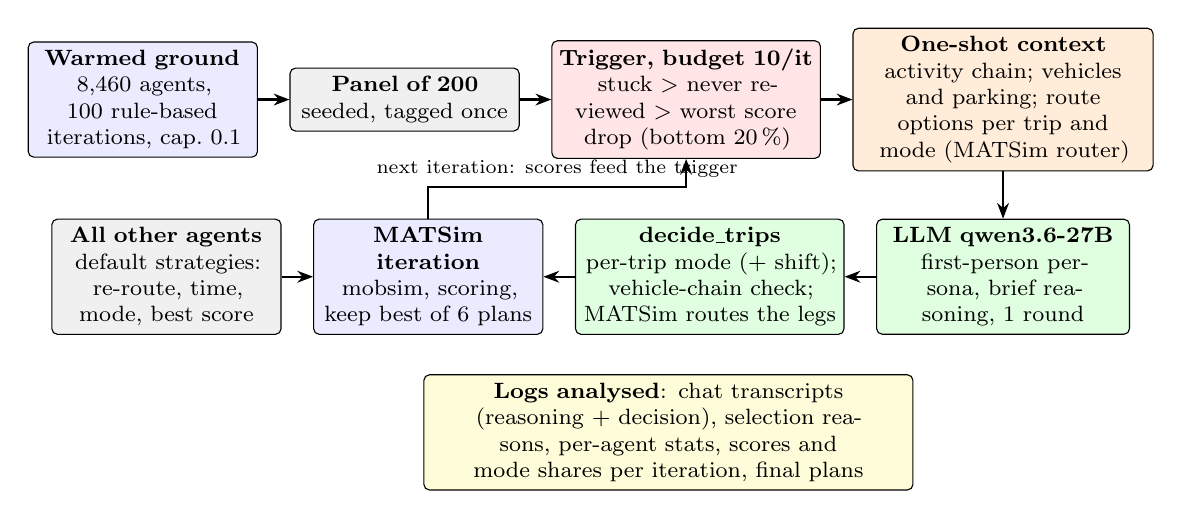
\begin{tikzpicture}[node distance=3mm and 4mm, font=\footnotesize,
  box/.style={draw, rounded corners=2pt, align=center, inner sep=3pt, minimum height=8mm, fill=#1},
  arr/.style={-{Stealth[length=2mm]}, thick}]
\node[box=blue!8, text width=27mm] (ground) {\textbf{Warmed ground}\\8,460 agents, 100 rule-based iterations, cap.\ 0.1};
\node[box=gray!12, text width=27mm, right=of ground] (panel) {\textbf{Panel of 200}\\seeded, tagged once};
\node[box=red!10, text width=32mm, right=of panel] (trig) {\textbf{Trigger, budget 10/it}\\stuck $>$ never reviewed $>$ worst score drop (bottom 20\,\%)};
\node[box=orange!15, text width=36mm, right=of trig] (ctx) {\textbf{One-shot context}\\activity chain; vehicles and parking; route options per trip and mode (MATSim router)};
\node[box=green!12, text width=30mm, below=6mm of ctx] (llm) {\textbf{LLM qwen3.6-27B}\\first-person persona, brief reasoning, 1 round};
\node[box=green!12, text width=32mm, left=of llm] (dec) {\textbf{decide\_trips}\\per-trip mode (+ shift); vehicle-chain check; MATSim routes the legs};
\node[box=blue!8, text width=27mm, left=of dec] (sim) {\textbf{MATSim iteration}\\mobsim, scoring, keep best of 6 plans};
\node[box=gray!12, text width=27mm, left=of sim] (rest) {\textbf{All other agents}\\default strategies: re-route, time, mode, best score};
\node[box=yellow!15, text width=60mm, below=5mm of sim.south west, anchor=north west, xshift=14mm] (log) {\textbf{Logs analysed}: chat transcripts (reasoning + decision), selection reasons, per-agent stats, scores and mode shares per iteration, final plans};
\draw[arr] (ground) -- (panel); \draw[arr] (panel) -- (trig); \draw[arr] (trig) -- (ctx); \draw[arr] (ctx) -- (llm); \draw[arr] (llm) -- (dec); \draw[arr] (dec) -- (sim);
\draw[arr] (rest) -- (sim);
\draw[arr] (sim.north) -- ++(0,4mm) -| node[pos=0.25, above, font=\scriptsize]{next iteration: scores feed the trigger} (trig.south);
\end{tikzpicture}
\caption{The loop. Ten panel agents per iteration are decided by the LLM; everyone else replans with MATSim's rules. Scoring is the same for all plans, so an LLM plan survives only if it scores well. Nothing about the outcome is fed back to the persona.}
\label{fig:scheme}
\end{figure}

\section{What was achieved}
\subsection{A reliable and fast protocol}
\begin{table}[h]\centering\small
\begin{tabular}{lrlr}\toprule
queries & 250 & decisions applied by MATSim & 250 \\
model rounds per query & 1 (all) & retries / verification failures / cap hits & 0 / 0 / 0 \\
wall time per query, median (max) & 39\,s (105\,s) & model resident / after a reload & 32\,s / 52\,s \\
LLM time: generation / prompt / load & 66 / 8 / 25\,\% & generation speed & 26 tokens/s \\
run wall time & 186\,min & iteration, median (min--max) & 6.4\,min (5.4--9.7) \\
\bottomrule\end{tabular}
\caption{Protocol and timing.}\label{tab:protocol}\end{table}

Every query ended with a valid decision in the first round; no agent was re-asked and no decision failed the chain check (Table~\ref{tab:protocol}). Query time is bimodal (Fig.~\ref{fig:timing}b): 32\,s with the model resident, 52\,s after a reload. The reloads are not ours: a colleague ran the same model with a smaller context during iterations 1--3 and 17--25, and Ollama reloads the 17\,GB weights on every switch (Fig.~\ref{fig:iterations}). A reload-free iteration takes 5.5\,min, of which 5.3\,min are the ten queries and 30\,s is MATSim. Compared with the tool-calling protocol of the previous runs (375\,s per agent, 6--9 rounds) this is a tenfold gain, obtained by pre-computing the facts and asking for a decision instead of a full plan.

\begin{figure}[h]\centering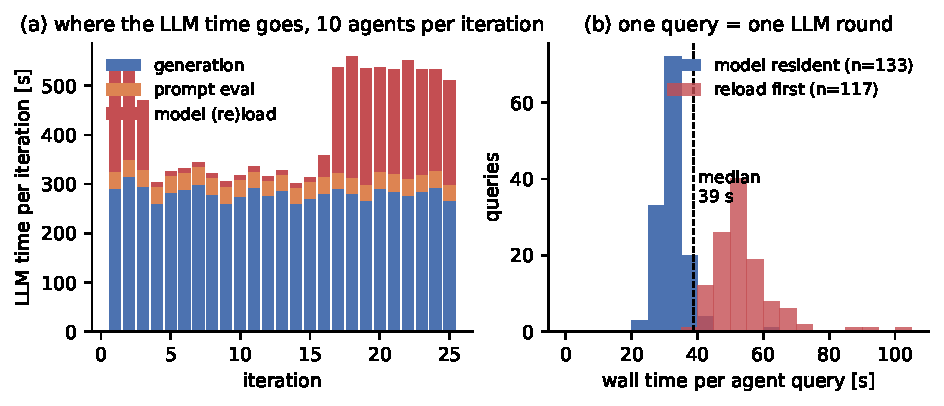
\includegraphics[width=0.85\textwidth]{fig_timing}
\caption{LLM time. (a) Per iteration, split into generation, prompt evaluation and model loading. (b) Wall time per query.}\label{fig:timing}\end{figure}
\begin{figure}[h]\centering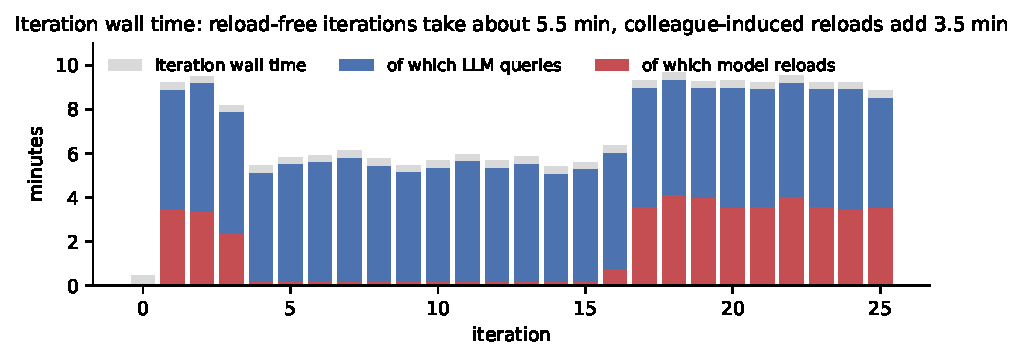
\includegraphics[width=0.85\textwidth]{fig_iterations}
\caption{Iteration wall time. Grey: whole iteration; blue: the ten LLM queries; red: the part spent reloading the model after another user's job.}\label{fig:iterations}\end{figure}

\subsection{The panel logic works and the ground stays at rest}
Iterations 1--20 reviewed all 200 panel agents once; from iteration 21 the trigger selected 50 agents by score drop (median drop 0.22 utils, maximum 4.25), so 39 agents were queried twice or more (Fig.~\ref{fig:decisions}c). Mean executed score moved from 20.157 to 20.166 over the run, mode shares by under one point, and no agent was stuck at the end (Fig.~\ref{fig:ground}). Ten decisions per iteration among 8,460 agents are invisible at population level. That is what a controlled instrument needs, and it is also why this run could not show behaviour (Section~\ref{sec:not}).

\begin{figure}[h]\centering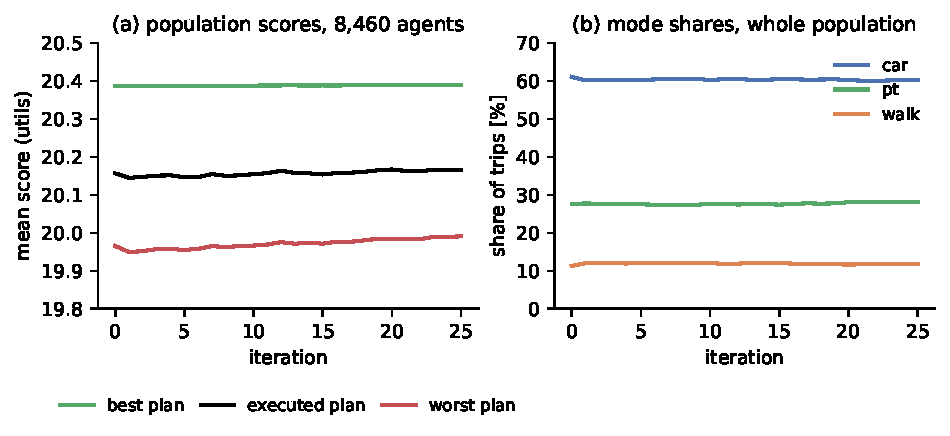
\includegraphics[width=0.8\textwidth]{fig_ground}
\caption{Ground health. (a) Mean score of the executed, best and worst plan. (b) Mode shares of all trips.}\label{fig:ground}\end{figure}

\subsection{A persona voice survives the short-reasoning instruction}
The traces speak in the first person (median 3.4 first-person markers per 100 words) and the detector counts the persona as ``emerged'' (first-person voice plus at least two grounded traits) in 195 of 250 conversations (Fig.~\ref{fig:persona}). Age is cited in 241 traces, car ownership in 197, employment in 52. No repetition loops, no contradiction between a stated trait and a decision (for example a carless agent choosing car).

\begin{figure}[h]\centering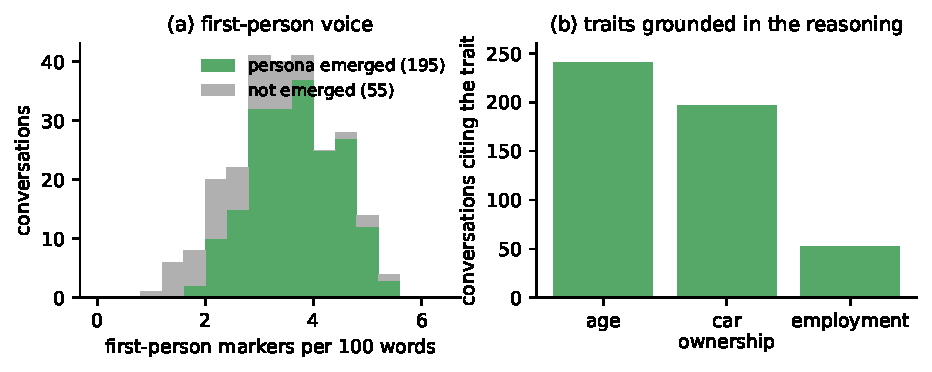
\includegraphics[width=0.78\textwidth]{fig_persona}
\caption{Persona signals in the reasoning traces. (a) First-person density. (b) Traits cited.}\label{fig:persona}\end{figure}

\section{What the model actually decides, and why}\label{sec:says}
\subsection{The decision is a rule}
The model kept the day in 191 of 250 queries and changed at least one trip in 59 (42 agents); 102 of 113 changed trips became car trips (Fig.~\ref{fig:decisions}). Reading the decisions against the agent's attributes and current modes removes the apparent variety (Fig.~\ref{fig:who}a): car owners switched 84 of their 86 bus trips and all 18 of their walk trips to car, and left all 270 car trips as they were; carless agents kept 105 of 112 bus trips (7 to walk) and 12 of 14 walk trips (2 to bus). Departure times were never touched. Whether the day changes is therefore decided by two facts, \emph{owns a car} and \emph{is not already driving}. Age and job appear in every trace but change nothing: the higher change rate of older car owners (Fig.~\ref{fig:who}b) is composition, older agents in this sample are more often on the bus. Re-selected agents confirm it: all 17 who had changed changed again (15 to car), 32 of 33 who had kept kept again.

\begin{figure}[h]\centering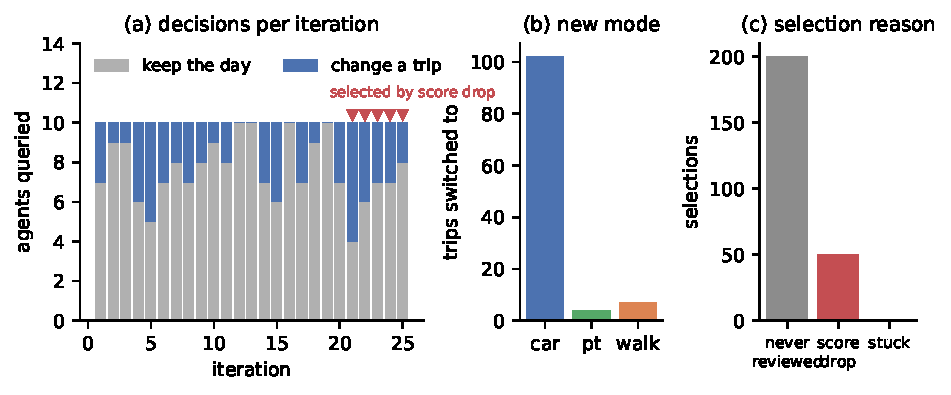
\includegraphics[width=0.85\textwidth]{fig_decisions}
\caption{Decisions. (a) Keep versus change per iteration; red markers: iterations with score-drop selection. (b) New mode of the 113 changed trips. (c) Selection reasons.}\label{fig:decisions}\end{figure}
\begin{figure}[h]\centering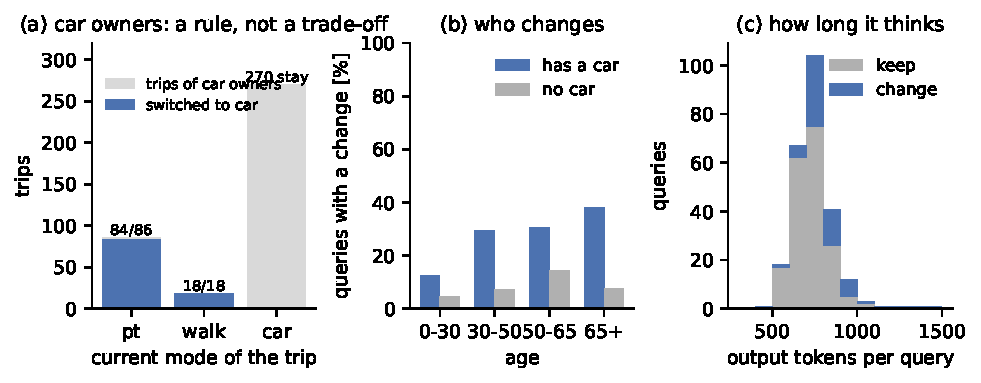
\includegraphics[width=0.88\textwidth]{fig_who}
\caption{Who changes. (a) Car owners' trips by current mode and whether they were switched to car. (b) Share of queries with a change, by age and car access. (c) Output tokens per query.}\label{fig:who}\end{figure}

\subsection{The switch ignores the numbers it was given}
Figure~\ref{fig:reasoning}b plots, for every bus trip of a car owner, the bus time against the car time the model was given. The switch happens on both sides of the diagonal: 14 of the 84 switches went to a car that is slower than the bus, by up to 33 minutes, and no car owner kept the bus when the car was faster. Transfers do not matter either: the switch rate is 6/6 at zero transfers, 69/71 at two, 9/9 at four. Over all 113 changed trips, 16 chose a mode slower than the current one (mean penalty 13 min). The persona's rule is ``I have a car, I drive'', stated in the language of comfort and age, and it overrides the travel times it was asked to weigh. The carless persona is the mirror image: it keeps the bus even for short trips, rejecting walking on distance and age.

\subsection{What the reasoning talks about}
Figure~\ref{fig:reasoning}a counts which considerations appear in the 250 traces (regular expressions over reasoning and answer). Travel time, the car-availability rule, age, transfers, employment and comfort are near universal; walking distance and reliability appear in about 60\,\%; weather in a third; parking in 22 traces; health in 11; money in 3. The persona never thinks about cost, which is the one term of MATSim's utility function that could have argued for the bus. Despite the instruction not to re-derive the numbers, 232 of 250 traces restate the given travel times in seconds and convert them to minutes before deciding; the median trace is 1,600 characters of reasoning followed by 800 characters of answer. Re-check loops (``Wait, ...'') are rare with the 3,072-token cap: two traces contain three or more, none hit the cap.

\begin{figure}[h]\centering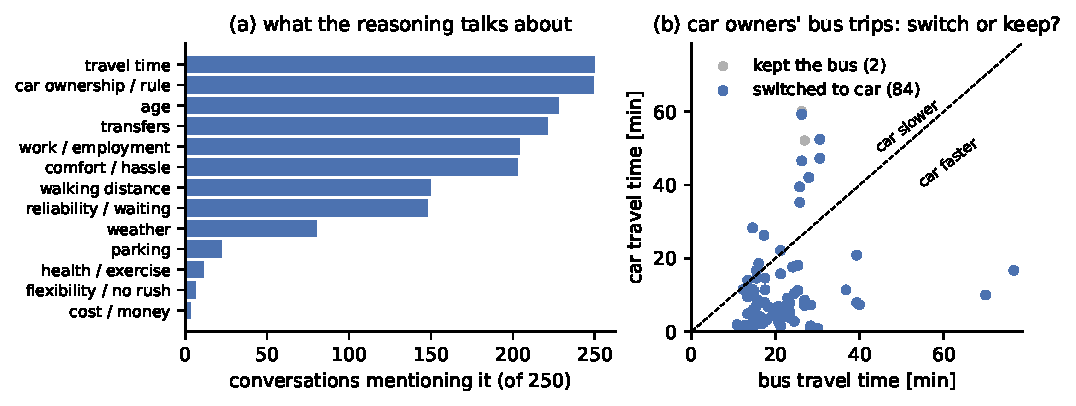
\includegraphics[width=0.88\textwidth]{fig_reasoning}
\caption{(a) Considerations mentioned in the reasoning traces. (b) Car owners' bus trips: bus time versus car time as given to the model, coloured by decision. The diagonal is equal time.}\label{fig:reasoning}\end{figure}

\subsection{In the model's words}
\begin{table}[h]\small\centering
\begin{tabularx}{\textwidth}{@{}>{\raggedright\arraybackslash}p{3.1cm}X@{}}\toprule
53, has a car, switched to car & ``Looking at this plan, I'm supposed to take public transport both ways with 4 transfers each time. That's a lot of walking around and waiting for connections, especially at my age. Four transfers means getting on and off multiple times, which is tiring.'' \\
76, no car, kept the bus & ``Looking at my day, I'm heading out from home at 11:17 to a secondary activity, staying until 12:32, then coming back home. That timing feels fine for me, a nice midday outing. I don't have a car or bike available, so my choices are really just public transport or walking.'' \\
43, no car, switched to walk & ``I'm struck by how many transfers the public transport trips involve. Trip 1 has 6 transfers and trip 2 has 8 transfers! That's exhausting, getting on and off buses or trains that many times, waiting at stops, dealing with connections.'' \\
80, no car, thinking trace & ``PT takes about 35 mins and involves transfers (2 transfers). Wait, the route options say transfers: 2 for PT. That means getting on/off multiple times, which can be tiring for an elderly person. But walking 45 minutes straight might also be tough. Actually, PT is faster and less physically demanding than walking 2.2 km.'' \\
\bottomrule\end{tabularx}
\caption{Representative answers. The voice is consistent and plausible; the decision behind it is the rule of Section~\ref{sec:says}.}
\end{table}

\subsection{Did the plans survive scoring?}
For the 42 agents whose day the model changed (Fig.~\ref{fig:survival}): 16 no longer hold a plan with the LLM's modes (it scored worst of six and was removed), 26 still hold one, and for 15 it is the best-scoring and executed plan. Among the 24 agents holding both kinds of plan the score difference is tiny: median $+0.05$ utils, 20 of 24 within $\pm0.5$. Under capacity 0.1 the car and bus plans of these commuters score about the same, so MATSim's selection is close to a coin toss and the verdict is neither confirmation nor rejection.

\begin{figure}[h]\centering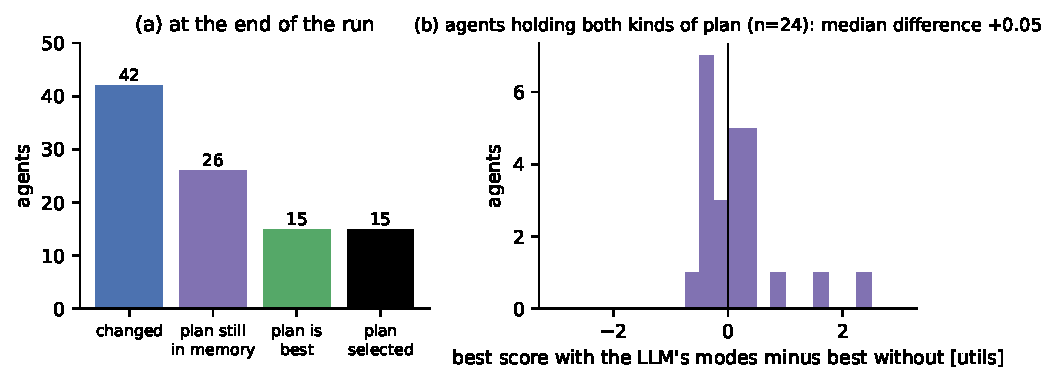
\includegraphics[width=0.85\textwidth]{fig_survival}
\caption{Fate of the 42 changed days at the end of the run. (a) Plans still in memory, best-scoring, executed. (b) Best score with the LLM's modes minus best without, for agents holding both.}\label{fig:survival}\end{figure}

\section{What was not achieved}\label{sec:not}
\textbf{No behavioural result.} Three design choices made the run flat: the LLM only proposes and MATSim's utility function judges, so a preference the utility does not share (avoiding transfers) is scored away; the ground was already at equilibrium, so there was nothing to improve and the score-drop trigger selected noise (0.2 utils); and 10 agents per iteration is 0.1\,\% of the population, too little for any network effect. The run characterises the instrument, not the phenomenon.

\textbf{No individuality.} The persona template gives the model three facts (age, employment, car access). The decision uses one of them. Everything else in the trace is narrative around a fixed rule. A population of such agents would be homogeneous within each car-access class, which is not what a persona approach is for.

\textbf{No learning.} The experience handler wrote 20,799 per-trip facts for the panel to the vector store during the run (``On day 6, the car trip from link 56\_4 to link 53\_1 took about 5 minutes 44 seconds during the afternoon peak''). None of them reached a prompt: 0 of 250 requests contained retrieved context. The retrieval code that handles a list of messages builds the enriched message and then discards it; whether the single-message path retrieved nothing for another reason is still to be checked. The persona therefore never saw yesterday's outcome or its own past decisions, which is why re-selected agents simply repeat themselves.

\textbf{No verdict from scoring.} Car and bus plans score alike for these agents, so the run cannot say whether the persona's rule is ``right'' in MATSim's terms. A rule-based control on the same panel is needed before the 15/42 survival can be interpreted.

\textbf{Tooling gaps.} The Python analysis suite reports 0\,\% success and 0 mode changes for this run because it looks for the old full-plan tool; the analyses above were done with two ad-hoc scripts kept next to this report. A departure-time change was never proposed, although the tool allows it.

\section{Issues found}
\textbf{A context bug that looked like a result.} The first attempt at this run was stopped after two iterations: 23 of 24 decisions were ``keep''. The context listed the modes available \emph{at each place under the current plan}; a car owner on the bus has the car at home, so the list said ``from work: walk, bus, passenger'' and the return trip had no car option. With the rule ``the car is wherever you last parked it'', the model concluded it could not drive home and did not drive out either. The fix presents vehicles at the level of the whole day, with the car option on every trip that an unbroken chain can bring it to, marked ``requires driving trip 1 as well''; the decision check follows the same chain. Same seed, same first ten agents: 0 changes before, 3 after (Fig.~\ref{fig:fix}). General lesson: a fact that is conditional on the plan being changed must be stated as a conditional, or the model reads it as a constraint.

\begin{figure}[H]\centering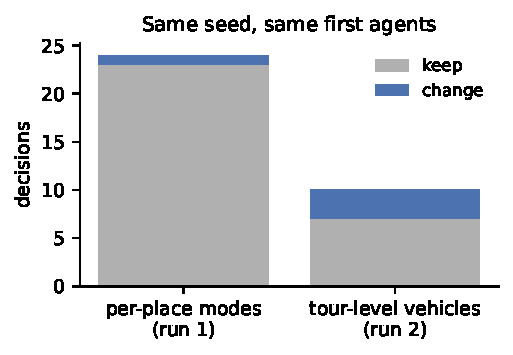
\includegraphics[width=0.38\textwidth]{fig_context_fix}
\caption{Same seed and first agents, before and after the context fix.}\label{fig:fix}\end{figure}

\textbf{Shared GPU.} A colleague's job using the same model name at another context size forced a reload in 117 of 250 queries, a quarter of all LLM time (Fig.~\ref{fig:iterations}). Our eviction script evicted by model name and could have unloaded their instance; it now checks the context size. \textbf{Innovation} was never switched off (the runner leaves MATSim's default), so the LLM ran in all 25 iterations; harmless here, to be decided for future runs. \textbf{The laptop} ran the MATSim side and had to stay open for three hours; moving it to the server is the remaining engineering step.

\section{Next}
\begin{enumerate}\setlength{\itemsep}{1pt}
\item \textbf{Final word for panel agents, with guards.} Panel agents keep only the LLM's plan; MATSim computes the consequences. The model still cannot judge feasibility, so the guards stay: the vehicle-chain check, MATSim routing, and a fallback to the previous plan if the executed day is stuck or infeasible. Then the population moves by what the personas decide.
\item \textbf{Experience in the loop.} Yesterday's realised travel times, delays and score change, plus the agent's own past decisions and reasons, injected as a short structured block (not raw transcripts), stored per agent in the vector store already in place. This is the mechanism for consistency \emph{and} for change.
\item \textbf{A shock, a cohort, a control.} Start from the warmed ground, remove a bus line or halve a corridor's capacity, decide a cohort of 100--200 agents by the LLM in the same iteration, with a rule-based cohort as control, and compare adaptation.
\item \textbf{Speed.} 32\,s per query is 745 generated tokens at 26 tokens/s. The levers, in order of gain: shorter or no reasoning on most queries (a decision alone is about 50 tokens, roughly 5\,s), our own model instance with parallel decoding on the server, and the 9B model for screening; the 27B with reasoning kept for a sample of queries so the persona metrics remain measurable.
\end{enumerate}
\end{document}
